\documentclass[twoside]{article}

\usepackage{subfigure, graphicx}
\usepackage[grid]{multicol}
\usepackage{listings, color}

\input{packs.tex}

%------------------------------------------------------------------------------
%	TITLE SECTION
%------------------------------------------------------------------------------
\title{\vspace{-15mm}\fontsize{24pt}{10pt}\selectfont\textbf{
    Synthesising a Compiler} } % Article title

\author{
  \large
  \textsc{Josh Reese}\\[2mm] % Your name
  \normalsize \href{mailto:jreese@cs.umd.edu}{jreese@cs.umd.edu}
  \vspace{-5mm}
}
\date{}

%------------------------------------------------------------------------------

\begin{document}
\maketitle % Insert title
\thispagestyle{fancy} % All pages have headers and footers

%------------------------------------------------------------------------------
%	ABSTRACT
%------------------------------------------------------------------------------

%% \begin{abstract}
%% \noindent \lipsum[1] % Dummy abstract text
%% \end{abstract}

%------------------------------------------------------------------------------
%	ARTICLE CONTENTS
%------------------------------------------------------------------------------
\begin{multicols}{2} % Two-column layout throughout the main article text

%-----------------------------------------------------------------------------
% INTRO
%------------------------------------------------------------------------------

\section{Introduction}
Reasoning about the functionality and properties of real programming
languages is a challenging and arduous task. In fact there are several
groups working on formally specifying the semantics of JavaScript for
various reasons \cite{js,ljs}. In some cases it is useful to have a
core language with well defined semantics to help reason about the
semantics of a more complicated, but related, language. However,
translating from one language to a simpler core is no trivial task.

Recent work in program synthesis shows very interesting results for
generating code that is able to fulfil previously defined
specifications \cite{flash,invert,sygus,feedback,sketch}. In this work
we hope to show that given the specifications for a compiler we will
be able to automatically generate code to translate from an
expressive, rich language with many features (i.e. lots of `syntactic
sugar' to a much more simple language which can be easily reasonable
about semantically. 

%------------------------------------------------------------------------------
% Methods
%------------------------------------------------------------------------------

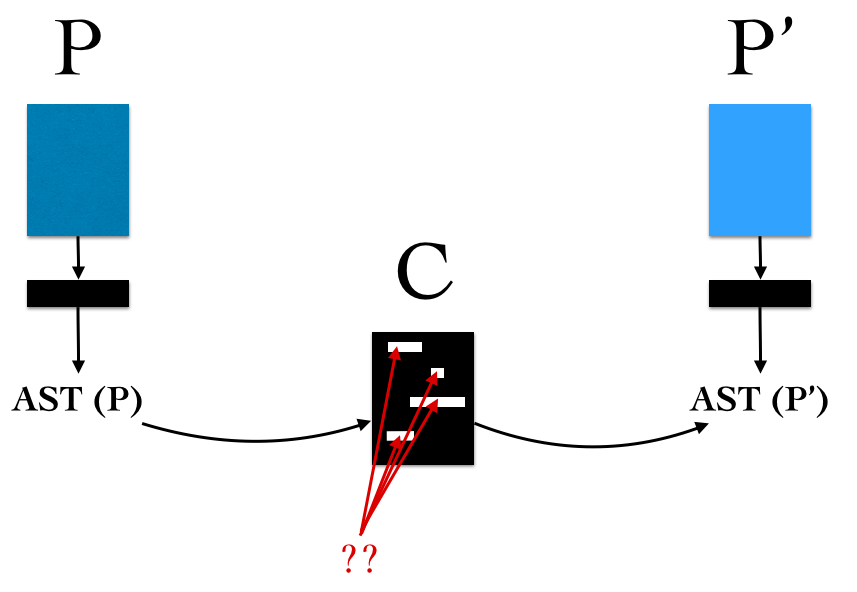
\includegraphics[width=\linewidth]{images/overview.png}
\captionof{figure}{Overview of translation of program $P$
  in language $L$ to program $P'$ in language $L'$}
\label{fig:overview}

\section{Methods}
In order to complete this work we will develop a system in Racket
\cite{racket} which will synthesise a compiler from some language $L$
toa language $L'$  where $L'$ $\subseteq$ $L$. In order to achieve this 
goal we will need to first identify target languages to use for
compilation. One potential target for the language $L'$  is to use
something akin to A-normal form (A-NF) \cite {anf} which will allow us
to use a functional language as $L$ that we can then transform to
A-NF. In order to accomplish this we will be working with ASTs which
represent programs in $L$  and $L'$. Once we have trees that represent
programs in our languages we can begin to synthesise transformations
from trees of type $L$ to trees of type $L'$. There has been extensive
work on tree transformations \cite{bek,fast} which we will hopefully
be able to draw from in order to automatically generate
transformations. \\\\The transformations we will be using are:
\begin{compactitem}
\item Delete node
\item Replace node
\item Swap nodes
\item Rotate (sub)tree
\item TODO: more?
\end{compactitem}

Our initial synthesis approach will be a brute-force search where we
apply all the transformations in various orders until a correct
transformation is found (or all possibilities are exhausted). In the
case of attempting all transformations with no successful result we
can conclude there is no possible transformation between these trees.

While this is certainly one way to approach this problem there has
been work on synthesis that tries to evaluate the `correctness' of an
attempted solution using various criteria
\cite{genprog,invert}. Building on these ideas we could apply some
transformation(s) to the ASTs, evaluate whether or not this was a
`good' transformation and use that to guide our searches.

A final possibility for guiding our searches is to perform a symbolic
search on the trees to help synthesise the appropriate
transformations. This will follow some of the ideas presented in
Rosette \cite{rosette}. This work is a framework for designing
languages which use SMT solvers. In addition to this it is embedded in
Racket which contributes to our decision for using Racket in our work.

A pictorial overview of this can be found in Figure
\ref{fig:overview} and a sample de-sugaring can be found in Listing
\ref{fig:cond}.

\lstset{basicstyle=\footnotesize,
  language=Lisp,
  morekeywords={cond-desug, if, else, <void>},
  keywordstyle=\bfseries\color{red},
  caption="De-sugaring Scheme's cond macro",
  label=fig:cond}

\begin{lstlisting}
  (cond cond-clause...)
  cond-clause =
        [test-expr then-body...+]
      | [else then-body...+]

  (cond-desug desug-clause...)
  desug-clause =
        [if test-expr (begin then-expr...+)
          #<void>]
      | [if #t (begin then-expr...+)
          #void]
\end{lstlisting}
%------------------------------------------------------------------------------
% Timeline
%------------------------------------------------------------------------------
\section{Timeline}
\begin{figure*}[ht!]
  \centering
  \subfigure[] {
    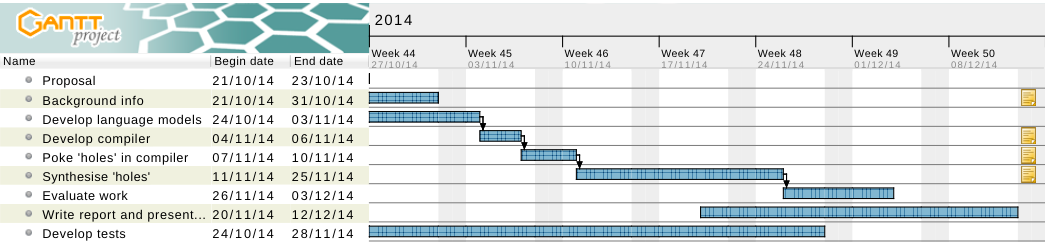
\includegraphics[width=\textwidth]{gantt/gantt_timeline.png}
    \label{fig:subgant0}
  }
  
  \subfigure[] {
    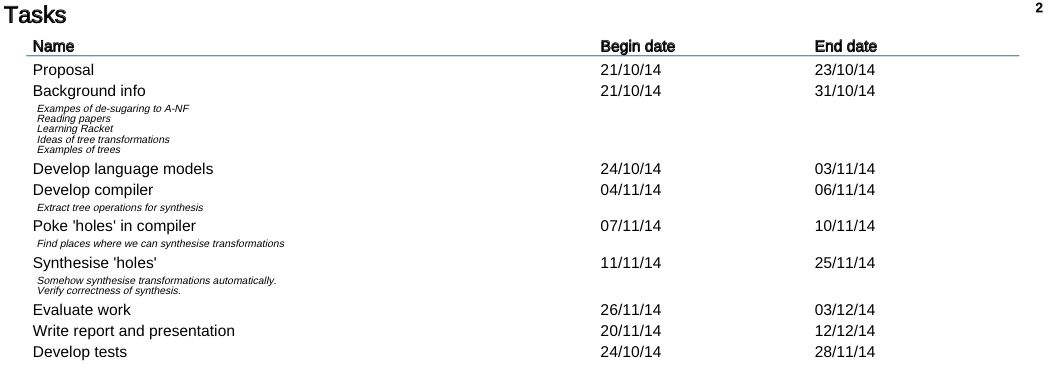
\includegraphics[width=\textwidth]{gantt/gantt_tasks.png}
    \label{fig:subgant1}
  }
  \caption [Gantt chart showing the prosed project time-line and notes.]
           {Figure \ref{fig:subgant0} shows the time-line of the
             project while Figure \ref{fig:subgant1} shows details
             about the tasks.}
  \label{fig:gantt}
\end{figure*}

In order to achieve the goals of this project we will need to complete
a series of tasks which involve: continued background research,
developing language models, developing a compiler for our languages,
poking holes in this compiler, synthesising these holes, and
evaluating our work. We have already been looking at papers related to
program synthesis, and will continue to do so, but we will need to
focus more on the specifics of the languages we are
targeting. Specifically what `sugared' syntax's we are interested in
`de-sugaring'. We will also need to determine a set of candidate tree
transformations that can be used in our synthesis. Once there is some
understanding regarding these concepts we can move on to developing
the language models in racket that we will be using. Following this we
can write the compiler for the language with holes in it. The real
challenge to the project comes next: synthesising the
transformations. This presents a number of challenges. One of which is
gathering input data to be used during synthesis. Since we will be
synthesising a tool which produces programs we will need to provide
correct programs as inputs (in language $L$) and their corresponding
correct programs as outputs (in language $L'$). Once this is finished
we can move on to evaluating our work and preparing the necessary
reports. A Gantt chart of the proposed time-line can be found in
Figure \ref{fig:gantt}.  

%------------------------------------------------------------------------------
% Evaluation
%------------------------------------------------------------------------------
\section{Evaluation}
Evaluation of the final product will fairly straightforward. In order
to test this we will write programs in language $L$, use our
synthesised compiler to translate them to language $L'$ and finally
verify their outputs are equivalent. If this is the case we have
succeeded. However, there are some subtle evaluation metrics that are
important to consider as well. These include: the time it takes to
synthesise a compiler for the language, how many language features the
synthesised compiler can handle, the quality of code produced among
others. All of these will need to be taken into account during
evaluation. Additionally, as previously mentioned, generating test
inputs for the synthesis process will prove a challenging task to
overcome. 



\bibliography{proposal}{}
\bibliographystyle{plain}


\end{multicols}

\end{document}
